\section{Przetwarzanie danych}\label{sec:przetwarzanie_danych}
\subsection{Zbiór początkowy}\label{subsec:zbior_poczatkowy}
Biblioteka \textit{pandas}\cite{mckinney-proc-scipy-2010} została użyta do wczytania danych z pliku \textit{csv} do obiektu \textit{DataFrame}.
Umożliwia ona łatwe i szybkie przetwarzanie danych, a także wygodne operacje na nich. Plik z danymi nie zawiera nagłówków, więc zostały one dodane ręcznie
poprzez ustawienie stałej \textit{HEADERS} jako listę nazw kolumn, w kolejności odpowiadającej kolejności kolumn w pliku z danymi.
Pierwsza kolumna \textit{lettr} jest etykietą klasy, a pozostałe to cechy.
\begin{figure}[H]
    \centering
    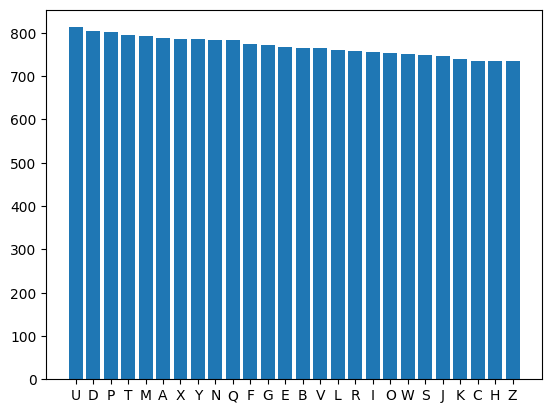
\includegraphics[width=0.8\textwidth]{img/bar_letter_count_initial.png}
    \caption{Początkowy rozkład klas w zbiorze danych.}
    \label{fig:bar_letter_count_initial}
\end{figure}
Najwięcej przykładów w zbiorze danych ma klasa \textit{U}, a najmniej \textit{Z}. 
Zbiór danych jest zbalansowany, ponieważ różnica między najczęściej i najrzadziej występującą klasą wynosi około 11\%.
Wizualnie na wykresie \ref{fig:bar_letter_count_initial} widać, że rozkład klas spada bardzo powoli z 813 do 734 przykładów.
\subsection{Filtrowanie danych}\label{subsec:filtrowanie_danych}
Zanim zbiór został podzielony na treningowy i testowy, został poddany filtrowaniu.
Dokonano najpierw usunięcia duplikatów, co zmniejszyło liczbę przykładów z 20 000 do 18 668.
Widoczny jest znaczący spadek liczby przykładów klasy \textit{I} która stała się najrzadziej występującą klasą.
\begin{figure}[H]
    \centering
    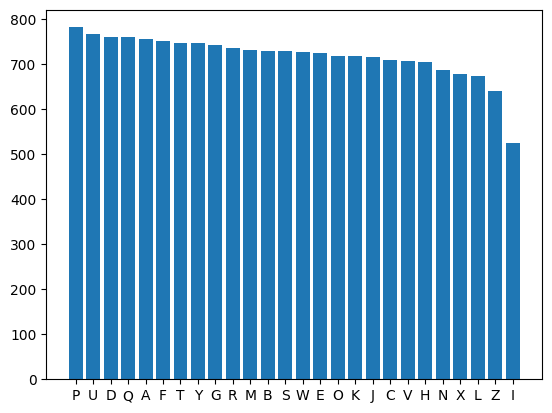
\includegraphics[width=0.8\textwidth]{img/bar_letter_count_duplicates.png}
    \caption{Rozkład klas w zbiorze danych po usunięciu duplikatów.}
    \label{fig:bar_letter_count_duplicates}
\end{figure}
Następnie usunięto przykłady odstające pomniejszające dalej do 17 257. Po tej operacji rozkład klas się zbliżył
do zbalansowanego, natomiast różnica między najczęściej i najrzadziej występującą klasą wynosi około 
43\% - znacznie więcej niż w zbiorze początkowym.
\begin{figure}[H]
    \centering
    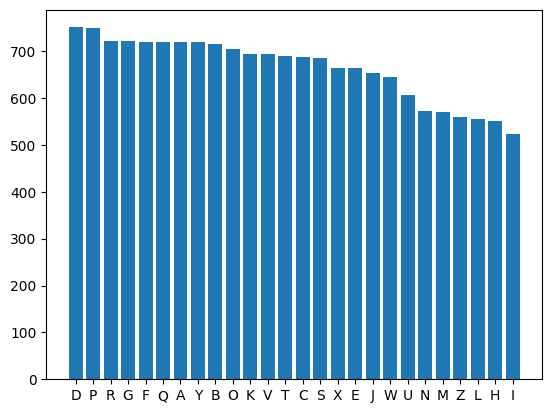
\includegraphics[width=0.8\textwidth]{img/bar_letter_count_outliers.png}
    \caption{Rozkład klas w zbiorze danych po usunięciu przykładów odstających.}
    \label{fig:bar_letter_count_outliers}
\end{figure}
\subsection{Balansowanie zbioru}\label{subsec:balansowanie_zbioru}
Wyżej wymieniona dysproporcja między najczęściej i najrzadziej występującą klasą może wpłynąć negatywnie na wyniki klasyfikacji.
Z tego powodu zastosowano techniki zrównywania liczebności klas: \textit{undersampling} i \textit{oversampling},
które odpowiednio zmniejszają i zwiększają liczebność klas. Undersampling zrównuje liczebność klas
poprzez usunięcie przykładów z pozostałych klas do liczby przykładów najrzadziej występującej klasy.
Oversampling działa przeciwnie, czyli generuje przykłady z pozostałych klas do liczby przykładów najczęściej występującej klasy.
Powstały 3 zbiory do przetestowania i wykorzystania w trenowaniu.
\subsection{Przygotowanie do trenowania}\label{subsec:przygotowanie_do_trenowania}
Zbiór danych został podzielony na treningowy i testowy w proporcji 80\% do 20\%
korzystając z wbudowanej metody \textit{train\_test\_split} biblioteki scikit-learn. Dzięki temu udało się uzyskać:
\begin{itemize}
    \item 15620 przykładów treningowych i 3906 testowych po oversamplingu
    \item 10878 przykładów treningowych i 2720 testowych po undersamplingu
    \item 13805 przykładów treningowych i 3452 testowych zbioru bez balansowania
\end{itemize}
Kolejnym krokiem było przekształcenie danych do postaci znormalizowanej, czyli takiej, w której cecha jest w granicach od 0 do 1.
W tym celu posłużono się metodą \textit{normalize} biblioteki scikit-learn.

